\chapter{Python and Basic Interfaces}
\section{Dataframes}
\noindent A dataframe is a data structure in \textit{pandas} that
allows multiple datasets to be mapped to the same indices. For
example, a data frame that maps dates to closing prices could be:

\begin{center}
  \begin{tabular}{lcccc}
    & \textbf{SPY} & \textbf{AAPL} & \textbf{GOOG} & \textbf{GLD}\\
    2000-01-09 & 100.01 & 50.89 & NaN & NaN\\
    2000-01-10 & 100.05 & 50.91 & NaN & NaN\\
    \vdots & \vdots & \vdots & \vdots & \vdots \\
    2015-12-31 & 200.89 & 600.25 & 559.50 & 112.37
  \end{tabular}
\end{center}

\noindent The indices in this dataframe are the dates on the left,
and the closing prices for that date are stored in each column. The
"NaN"s appear because \textit{GOOG} and \textit{GLD} were not
publicly traded during those periods.

\subsection{Reading CSVs into Dataframes}
\noindent To begin using the dataframes, you need data first.
Historical stock data from Yahoo is provided in the form of a CSV
file, which can be easily read into a dataframe using
\textit{pandas}'s function \textit{read\_csv()}.\\

\noindent
\begin{minipage}{\linewidth}
  \noindent\textit{example 1:}
  \lstinputlisting[style=python]{code_examples/dataframes_1.py}
\end{minipage}

\noindent This example reads in a CSV corresponding to the historic
data for \textit{AAPL} (Apple, Inc) into the variable \textit{df}.
\textit{df} is a \textit{DataFrame} object, which means any
\textit{DataFrame} methods may be used on it.\\

\noindent
\begin{minipage}{\linewidth}
  \noindent\textit{example 2:} An example of a method that can be
  used is \textit{max()}, which returns the maximum value in the range.\\
  \lstinputlisting[style=python]{code_examples/dataframes_2.py}
\end{minipage}

\subsection{Plotting}
\noindent \textit{Matplotlib} can be used to plot the data in the
dataframes, as pandas can conveniently tap into the
\textit{matplotlib} API. Plotting data in a dataframe is as simple as
calling \textit{plot()} on one of the series in the frame.\\

\noindent
\begin{minipage}{\linewidth}
  \noindent\textit{example 3:} Plotting the Adjusted
  Close\footnote{Adjusted Close is a historically-adjusted value of
    the stock that takes into account corporate actions (such as stock
  splits) and distributions (such as dividends issued).} price of \textit{AAPL}
  \lstinputlisting[style=python]{code_examples/dataframes_3.py}
\end{minipage}

\begin{figure}
  \centering
  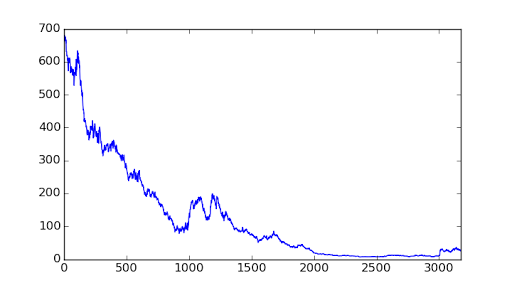
\includegraphics[width=\textwidth]{images/adj_close.png}
  \caption{Plot of adjusted close price for \textit{IBM} over all
    time. Notice that the indices are just numbers rather than dates
  and the plot goes backwards in time to the right}
\end{figure}

\noindent
\begin{minipage}{\linewidth}

  \noindent\textit{example 4:} Plotting multiple columns is as simple
  as adding a more entries to the selection statement

  \lstinputlisting[style=python]{code_examples/dataframes_4.py}
\end{minipage}

\subsection{Issues}
\noindent There are some issues with the data that need to be solved
to effectively use it in the way we want.

\paragraph{Trading days} The NYSE only trades for a certain number of
days per year, which means that indexing by dates will return some
results when the exchanges were not open. This poses problems for
trying to pull out certain date ranges from the dataframe.

\paragraph{Multiple stocks} One of the dataframe's powers is to be
able to contain multiple ranges, which means that we need to be able
to retrieve multiple datasets and store them into the dataframe.

\paragraph{Date order} The data in the Yahoo CSV are in reverse
chronological order (most recent at the top), so any analysis on the
dataframe will be going backwards in time, which is not ideal.

\subsection{Solution to the issues}
\noindent To solve the trading days problem, we'll use an \ac{etf}
called \textit{SPY} (S\&P 500) to serve as a basis for what days the
stock market is open. The only days that exist in the dataset for
this \ac{etf} are the days the stock market traded, so if we use this
as a reference and use joining on the dataframes, we can recover data
on only the days which had trading.\\

\noindent
\begin{minipage}{\linewidth}
  \noindent\textit{example 5:} Using joins to get only traded days

  \lstinputlisting[style=python,firstline=1,lastline=7]{code_examples/dataframes_5.py}
\end{minipage}

\noindent If we were to print out df1, the output would be:
\begin{lstlisting}[style=python]
Empty DataFrame
Columns: []
Index: [2010-01-22 00:00:00, 2010-01-23 00:00:00, 2010-01-25 00:00:00, 2010-01-26 00:00:00]
\end{lstlisting}

\noindent This empty dataframe will be the basis for the data we want
to retrieve.

\noindent The next step is to join this dataframe with a dataframe
with the data for \textit{SPY}. This will keep only indices of the
\textit{SPY} dataframe that also exist in the empty one.\\

\noindent
\begin{minipage}{\linewidth}
  \noindent\textit{example 6:} Reading in the new dataframe and joining them

  \lstinputlisting[style=python,firstnumber=8,firstline=8,lastline=11]{code_examples/dataframes_5.py}
\end{minipage}

\noindent
\begin{minipage}{\linewidth}
  \noindent The output would now be:
\begin{lstlisting}[style=python]
        Adj Close
2010-01-22    104.34
2010-01-23    NaN
2010-01-24    NaN
2010-01-25    104.87
2010-01-26    104.43
\end{lstlisting}
\end{minipage}

\noindent To get rid of the "NaN"s, you can call \textit{dropna()} on
the newly joined dataframe, but there is a better way of joining them
such that the "NaN"s don't appear in the first place. The join type
is called an \textit{inner} join, which joins at the intersection of
the two dataframes. This way, only the dates which are in both will
be kept as indices. Everything else will be thrown away.\\

\noindent
\begin{minipage}{\linewidth}
  \noindent\textit{example 7:} The inner join

  \lstinputlisting[style=python,firstline=16,lastline=16]{code_examples/dataframes_5.py}
\end{minipage}

\subsection{Multiple stocks}
\noindent Reading in multiple stocks is as easy as just adding a for loop:\\

\noindent
\begin{minipage}{\linewidth}
  \noindent\textit{example 8:} Reading in multiple stocks into a
  single dataframe

  \lstinputlisting[style=python,firstline=19,lastline=28]{code_examples/dataframes_5.py}
\end{minipage}

\noindent
\begin{minipage}{\linewidth}
  \noindent Here's an example of reading and plotting multiple
  stocks' closing price on one plot\\
  \noindent\textit{example 9:} Reading and plotting multiple stocks

  \lstinputlisting[style=python,firstline=31,lastline=77]{code_examples/dataframes_5.py}
\end{minipage}

\begin{figure}
  \centering
  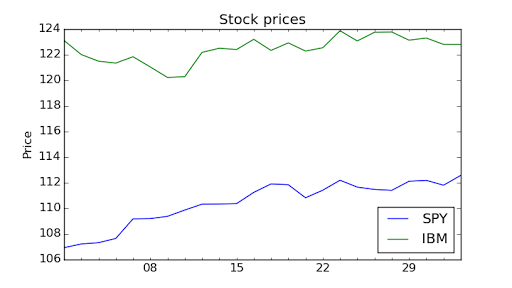
\includegraphics[width=\textwidth]{images/adj_close_mar.png}
  \caption{Plot of adjusted close price for \textit{IBM} and
  \textit{spy} over the month of April 2010}
\end{figure}

\subsection{Normalizing}
\noindent Sometimes when plotting, the values of a stock will be
significantly different from the other stocks such that it becomes
difficult to tell some of them apart. Normalizing the data allows all
of them to start at the same point and then show divergences from the
initial point, making it easier to compare them at the same time.\\

\noindent Normalizing the dataframe is as simple as dividing the
entire dataframe by its first row
\noindent
\begin{minipage}{\linewidth}
  \noindent\textit{example 10:} Normalizing a dataframe

  \lstinputlisting[style=python,firstline=81,lastline=83]{code_examples/dataframes_5.py}
\end{minipage}

\begin{figure}[h]
  \centering
  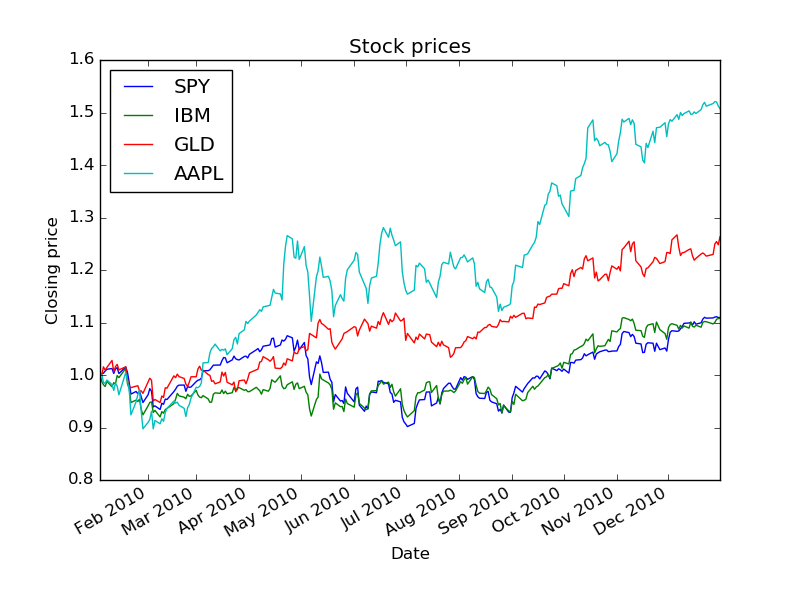
\includegraphics[width=\textwidth]{images/adj_close_normalized.png}
  \caption{Normalized stock prices over the year 2010}
\end{figure}
\newpage

\section{NumPy}

\noindent The actual data in the dataframe is actually an \textit{ndarray} in NumPy (A multidimensional homogeneous array). That means we can do operations on the data using NumPy. For example, if you have a dataframe \textit{df1}, the \textit{ndarray} would be extracted by doing

\begin{lstlisting}[style=python]
nd1 = df1.values
\end{lstlisting}

\noindent Accessing a cell in the array is as simple as:

\begin{lstlisting}[style=python]
val = nd1[row,col]
\end{lstlisting}

\noindent You can also access subarrays by indexing with the colon:

\begin{lstlisting}[style=python]
sub = nd1[0:3,1:3]
\end{lstlisting}

\noindent would capture the rectangular subarray from the first to the third rows and the second to third columns.

\paragraph{Indexing} Note that the second part of the index is 1 past the actual index that will be the last, so 0:3 only pulls out 0,1, and 2.

\noindent Like in MATLAB, you can pull out everything using just the colon. For example:

\begin{lstlisting}[style=python]
sub = nd1[3,:]
\end{lstlisting}

\noindent would retrieve all columns of row 3.

\paragraph{Negative indexing} To get the last index, you can use negative numbers (the last index would be -1, second to last -2, etc.)

\begin{lstlisting}[style=python]
sub = nd1[-1,1:3]
\end{lstlisting}

\noindent would get columns 1,2 of the last row.

\paragraph{Boolean indexing/masking} Suppose we want to get the values in an array, $a$, which are all less than the mean. NumPy's masking feature makes it really intuitive, as all you need to do is:

\begin{lstlisting}[style=python]
lessThanMean = a[a<a.mean()]
\end{lstlisting}

\noindent The array $a < a.mean()$ would be a boolean array, which might look like
\begin{lstlisting}[style=python]
[[True, True, False, False]]
\end{lstlisting}

\paragraph{Assignment} Assigning values in an array is easy using the NumPy notation. For example, say we wanted to replace the values in the first 2x2 square of \textit{nd1} with the 2x2 square in nd2 with columns 2 and 3, and rows 3, and 4. The operation would be:

\begin{lstlisting}[style=python]
nd1[0:2,0:2] = nd2[-2:,2:4]
\end{lstlisting}

\paragraph{Creating an array} Creating a numpy array is as easy as passing in a normal python list into the array method:

\begin{lstlisting}[style=python]
import numpy as np

print np.array([1,2,3])
\end{lstlisting}

\noindent Creating a 2D $mxn$ array is as simple as passing in a $m$-long list of $n$-tuples.

\begin{lstlisting}[style=python]
import numpy as np

print np.array([(1,2,3),(4,5,6)])
\end{lstlisting}

\noindent would output

\begin{lstlisting}[style=python]
[[1,2,3]
 [4,5,6]]
\end{lstlisting}

\paragraph{More initializers} You can also create arrays with certain initial values.

\begin{lstlisting}[style=python]
np.empty((5,3,2))
\end{lstlisting}

\noindent initializes an "empty" $5x3x2$ dimensional array. The values in the array are actually whatever was in the memory locations of the array pointers, so the output could look like garbage.

\begin{lstlisting}[style=python]
np.ones((5,4), dtype=np.int)
\end{lstlisting}

\noindent creates a $5x4$ array, where the value in each cell is the integer 1.

\begin{lstlisting}[style=python]
np.random.random((5,4))
\end{lstlisting}

\noindent creates a $5x4$ array with random numbers from a uniform distribution in [0.0,1.0). An example result could be:

\begin{lstlisting}[style=python]
[[ 0.82897637  0.36449978  0.91209931  0.96307279]
 [ 0.63777312  0.24482194  0.5817991   0.18043012]
 [ 0.85871221  0.98874123  0.68491831  0.53831711]
 [ 0.52908238  0.81083147  0.97440602  0.81032768]
 [ 0.98566222  0.38902445  0.16922005  0.0873198 ]]
\end{lstlisting}

\noindent Other methods or fields, such as $sum()$ or $size$ can be looked up in online documentation.